%----------------------------------------------------------------------------------------
%	PACKAGES AND OTHER DOCUMENT CONFIGURATIONS
%----------------------------------------------------------------------------------------

\documentclass[paper=a4, fontsize=11pt]{scrartcl} % A4 paper and 11pt font size

% ---- Entrada y salida de texto -----

\usepackage[T1]{fontenc} % Use 8-bit encoding that has 256 glyphs
\usepackage[utf8]{inputenc}
%\usepackage{fourier} % Use the Adobe Utopia font for the document - comment this line to return to the LaTeX default

% ---- Idioma --------

\usepackage[spanish, es-tabla]{babel} % Selecciona el español para palabras introducidas automáticamente, p.ej. "septiembre" en la fecha y especifica que se use la palabra Tabla en vez de Cuadro

% ---- Otros paquetes ----
\usepackage{csquotes} %Para permitir el uso de comillas Quotes https://tex.stackexchange.com/questions/36812/isnt-there-any-other-way-of-doing-double-quotes-in-latex-besides
\usepackage[hyphens]{url} % ,href} %para incluir URLs e hipervínculos dentro del texto (aunque hay que instalar href)
\usepackage{hyperref}
\usepackage{color}
\usepackage{graphics,graphicx, floatrow} %para incluir imágenes y notas en las imágenes
\usepackage{graphics,graphicx, float} %para incluir imágenes y colocarlas

\graphicspath {{./img/}}

\usepackage{listings}  %para introducir comandos

\lstdefinestyle{mybash}
{basicstyle=\ttfamily,
  showstringspaces=false,
  commentstyle=\color{red},
  keywordstyle=\color{blue},
  language=bash,
  alsoletter=/,
  basicstyle=\footnotesize,
  numbers=left,
  stepnumber=1,
  showstringspaces=false,
  tabsize=1,
  breaklines=true,
  breakatwhitespace=false,
}
\lstdefinestyle{mysql}
{basicstyle=\ttfamily,
  showstringspaces=false,
  commentstyle=\color{red},
  keywordstyle=\color{blue},
  language=sql,
  basicstyle=\footnotesize,
  numbers=left,
  stepnumber=1,
  showstringspaces=false,
  tabsize=1,
  breaklines=true,
  breakatwhitespace=false,
}


% Para hacer tablas comlejas
%\usepackage{multirow}
%\usepackage{threeparttable}

%\usepackage{sectsty} % Allows customizing section commands
%\allsectionsfont{\centering \normalfont\scshape} % Make all sections centered, the default font and small caps

\usepackage{fancyhdr} % Custom headers and footers
\pagestyle{fancyplain} % Makes all pages in the document conform to the custom headers and footers
\fancyhead{} % No page header - if you want one, create it in the same way as the footers below
\fancyfoot[L]{} % Empty left footer
\fancyfoot[C]{} % Empty center footer
\fancyfoot[R]{\thepage} % Page numbering for right footer
\renewcommand{\headrulewidth}{0pt} % Remove header underlines
\renewcommand{\footrulewidth}{0pt} % Remove footer underlines
\setlength{\headheight}{13.6pt} % Customize the height of the header

\setlength\parindent{0pt} % Removes all indentation from paragraphs - comment this line for an assignment with lots of text

\newcommand{\horrule}[1]{\rule{\linewidth}{#1}} % Create horizontal rule command with 1 argument of height


%----------------------------------------------------------------------------------------
%	TÍTULO Y DATOS DEL ALUMNO
%----------------------------------------------------------------------------------------
\graphicspath{ {img/} }

\title{
\normalfont \normalsize

\includegraphics[width=6cm,height=6cm]{logo}\\
\textsc{\textbf{Bootcamp Especialidad GNU/Linux (2023)}} \\ [25pt] % Your university, school and/or department name(s)
\horrule{0.5pt} \\[0.4cm] % Thin top horizontal rule
\huge Lab 08 - Instalación de Phpmyadmin \\ % The assignment title
\horrule{2pt} \\[0.5cm] % Thick bottom horizontal rule
}

%https://es.overleaf.com/learn/latex/Inserting_Images
%Ruta relativa de   imagenes

\author{Pedro Antonio Mayorgas Parejo} % Nombre y apellidos

\date{\normalsize\today} % Incluye la fecha actual

%----------------------------------------------------------------------------------------
% DOCUMENTO
%----------------------------------------------------------------------------------------

\begin{document}

\maketitle % Muestra el Título

\newpage %inserta un salto de página

\tableofcontents % para generar el índice de contenidos

\newpage

%----------------------------------------------------------------------------------------
%	Cuestión 1
%----------------------------------------------------------------------------------------

\section{Notas}

Se ha reutilizado la máquina de la entrega del laboratorio 7, para no tener que reinstalar MariaDB server.
\vspace{5mm}

Usualmente la instalación de phpmyadmin con Apache2 es más directa que nginx, así que lo haremos en nginx para poder ver cómo los componentes trabajan juntos.

\section{Instalación}

Para instalar Phpmyadmin, simplemente tenemos que ejecutar los siguientes comandos:

\begin{lstlisting}[style=mybash]
sudo apt update && sudo apt dist-upgrade -y
sudo apt install phpmyadmin nginx php-fpm
\end{lstlisting}

El paquete \textbf{php-fpm}, es necesario para que nginx pueda trabajar con phpmyadmin, ya que este no tiene como en apache2, un módulo directo que le retorne los HTML que debe pasar por HTTP.

\begin{figure}[H]
	\centering
	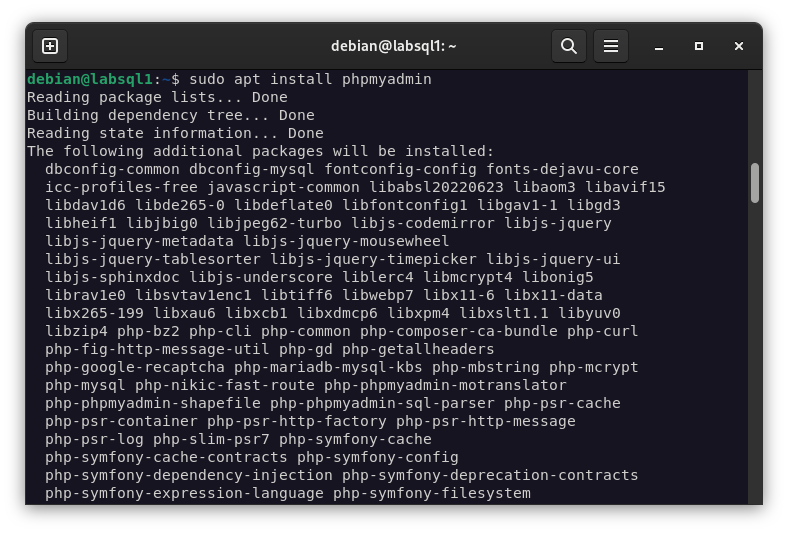
\includegraphics[scale=0.30]{00}
	\caption{Instalación de phpmyadmin, dependencias necesarias.}
\end{figure}

Durante la instalación nos preguntará si queremos configurarlo para Apache2, o para lighthttpd. No marcamos ninguna opción y luego nos pedirá la configuración de una contraseña para una base de datos que debe ser alojada por el phpmyadmin para sus configuraciones.

\begin{figure}[H]
	\centering
	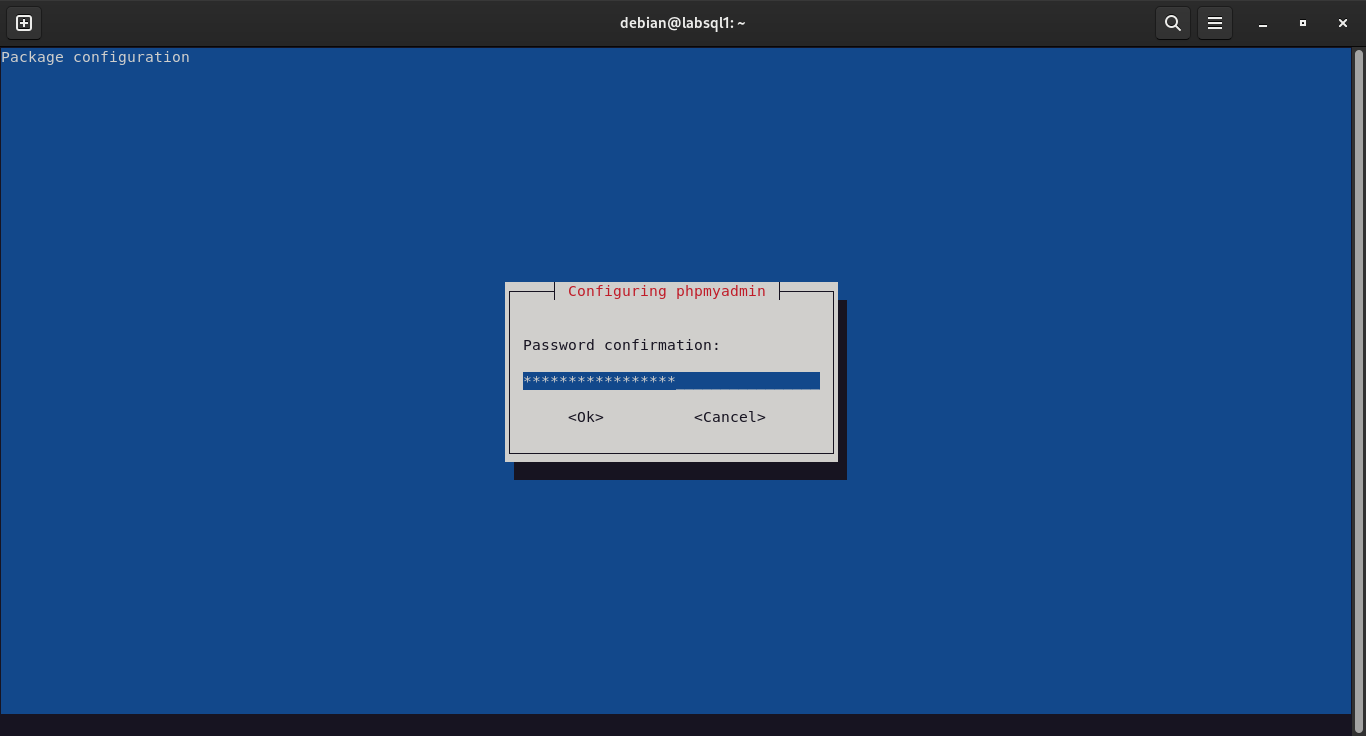
\includegraphics[scale=0.30]{01}
	\caption{Configuración de la contraseña de Phpmyadmin.}
\end{figure}

\begin{figure}[H]
	\centering
	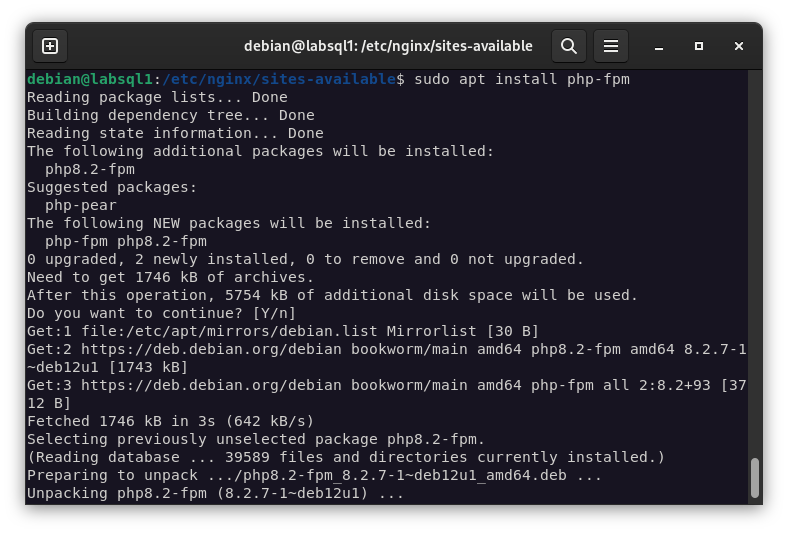
\includegraphics[scale=0.30]{02}
	\caption{Instalación de php-fpm, dependencias necesarias.}
\end{figure}

\begin{figure}[H]
	\centering
	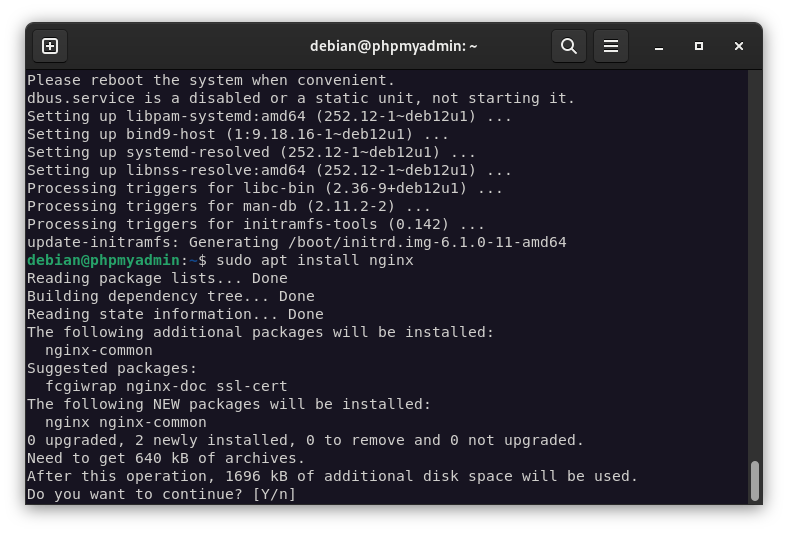
\includegraphics[scale=0.30]{03}
	\caption{Instalación de nginx, dependencias necesarias.}
\end{figure}

Una vez que lo tenemos todo instalado, si accedemos al virtualhost principal, lo que veremos es la página de nginx y además dentro de \textbf{/etc/nginx/sites-available}, no hay otro fichero de configuración disponible asociado a phpmyadmin. Por lo que tendremos que crearlo manualmente a partir del default. 
\vspace{5mm}

Otro punto a tener en cuenta, es que el directorio de phpmyadmin, no está en el directorio donde se sirven las webs por parte del servicio web \textbf{/var/www/}, por lo que debemos crear un enlace simbólico desde donde existen dichos ficheros de configuración que están localizados en \textbf{/usr/share/phpmyadmin}.

\begin{figure}[H]
	\centering
	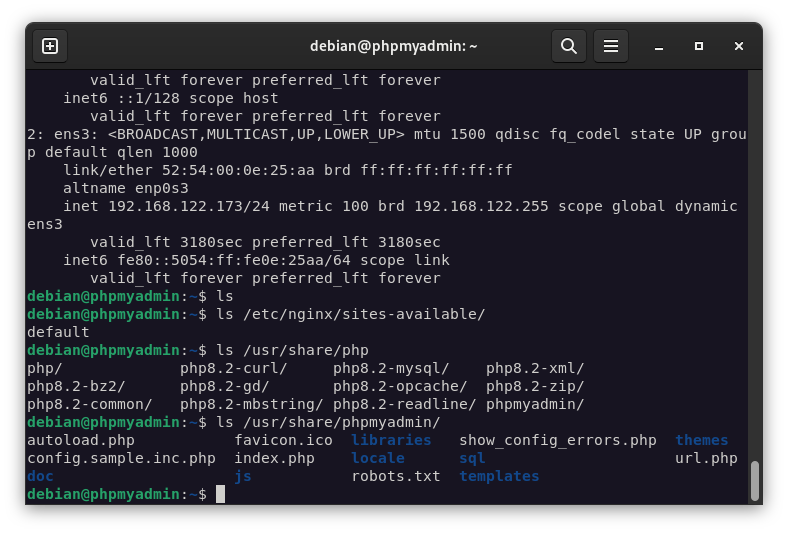
\includegraphics[scale=0.30]{05}
	\caption{Localización de los ficheros de configuración y de phpmyadmin.}
\end{figure}

Como primer paso, vamos a preparar los directorios de phpmyadmin para que estén listos para ser servidos. Para ello ejecutamos los siguientes comandos:

\begin{lstlisting}[style=mybash]
sudo rm -rf /var/www/*
sudo ln -s /usr/share/phpmyadmin /var/www/
# Listamos el directorio /var/www para ver si el enlace simbolico se ha realizado correctamente
sudo chown -R www-data:www-data /var/www/phpmyadmin
\end{lstlisting}

\begin{figure}[H]
	\centering
	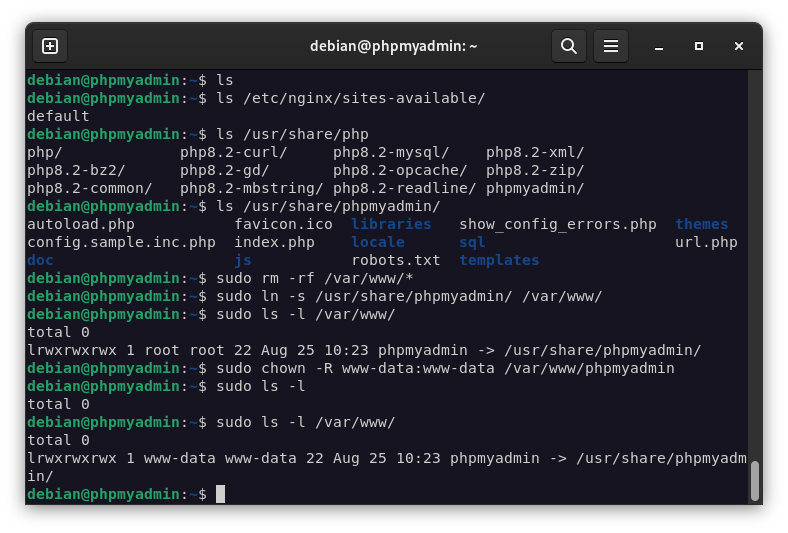
\includegraphics[scale=0.30]{06}
	\caption{Creación del enlace simbólico del directorio de phpmyadmin.}
\end{figure}

Ahora tenemos que configurar el fichero del virtualhost default que está localizado en \textbf{/etc/nginx/sites-available/default}, para poder hacer funcionar el phpmyadmin, así como que tenga su intérprete php-fpm y su nombre \textbf{mybddd.com}. Además debemos cambiar la versión de php-fpm, ya que esta es mas moderna que la que está en el fichero.

\begin{figure}[H]
	\centering
	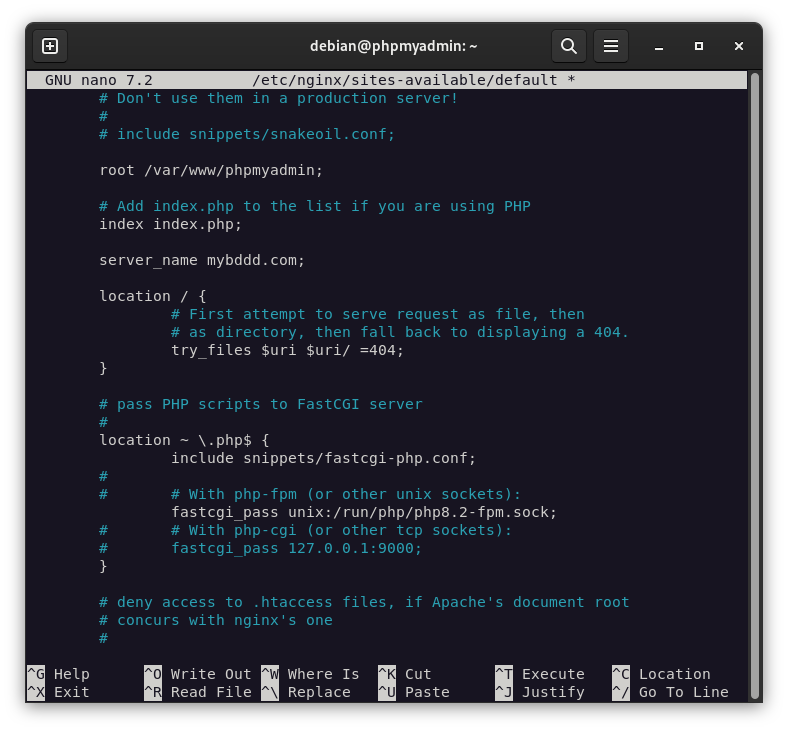
\includegraphics[scale=0.30]{07}
	\caption{Edición del fichero default.}
\end{figure}

Luego de editar el fichero de default, tenemos que reiniciar el servicio y verificar que su estado esté correcto, en otro caso podría haberse producido un error a la hora de editar el fichero de configuración.

\begin{figure}[H]
	\centering
	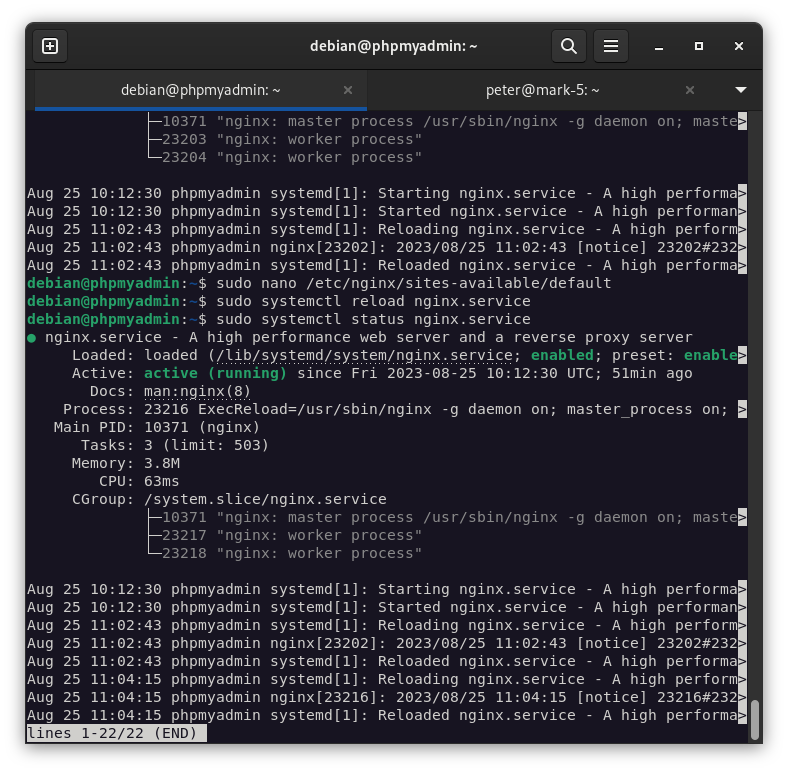
\includegraphics[scale=0.30]{10}
	\caption{Reiniciando el servicio de nginx.}
\end{figure}

\begin{lstlisting}[style=mybash]
sudo systemctl restart nginx.service
sudo systemctl status nginx.service
\end{lstlisting}

\begin{figure}[H]
	\centering
	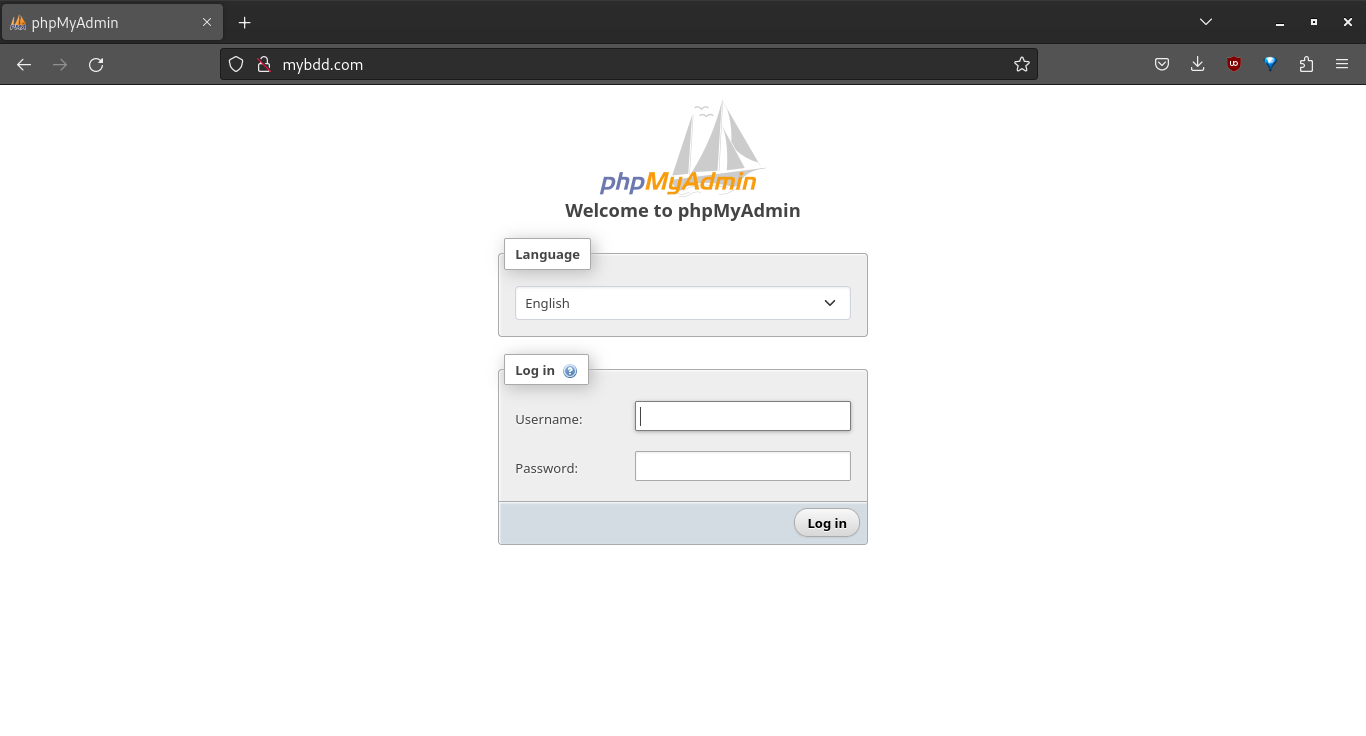
\includegraphics[scale=0.30]{08}
	\caption{Entrando en phpmyadmin.}
\end{figure}

Para la actividad hemos generado un usuario y una base de datos vacía. La tabla ha sido creada con phpmyadmin.
\begin{figure}[H]
	\centering
	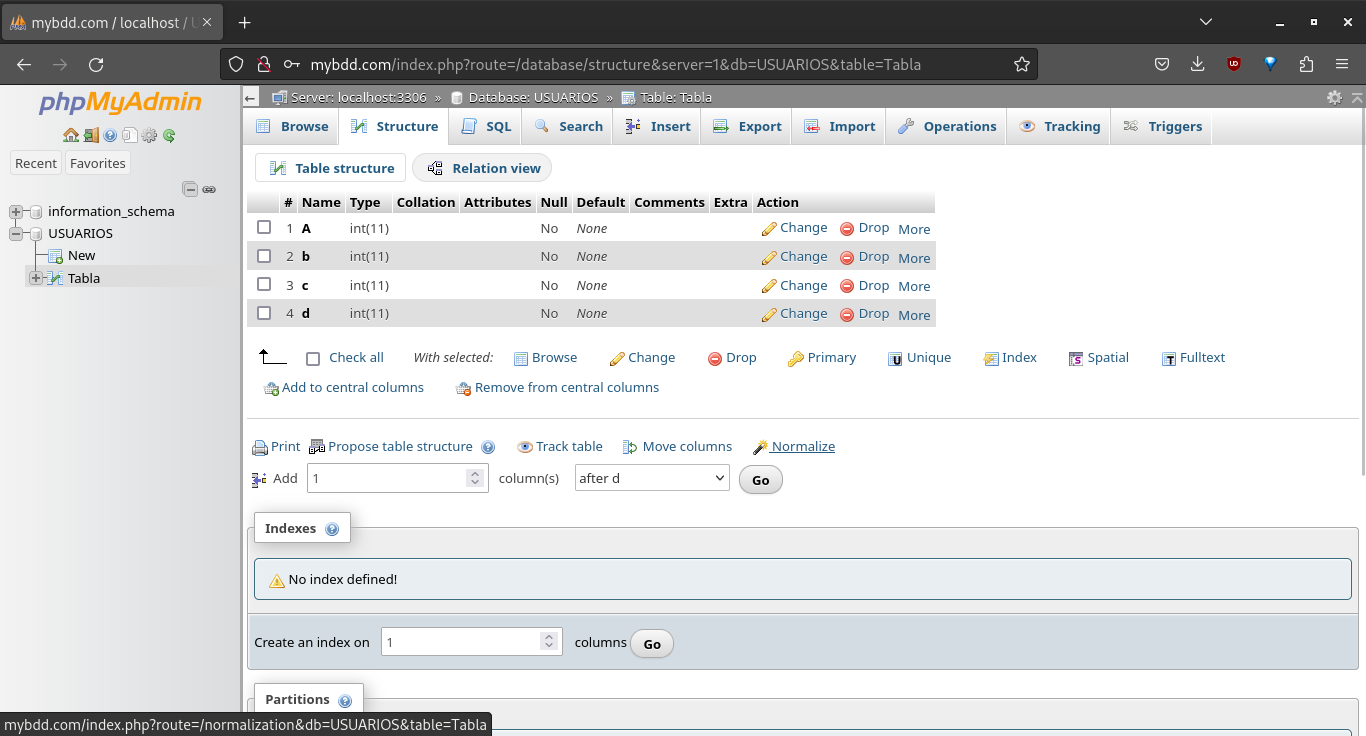
\includegraphics[scale=0.30]{09}
	\caption{Tabla del usuario en la base de datos de USUARIOS.}
\end{figure}
% \vspace{5mm}


% \begin{lstlisting}[style=mybash]
%     # Para una base de datos concreta
%     mysqldump --user=tiendabd --password=password --databases tiendabd --add-drop-database --add-drop-table [--replace] --host=127.0.0.1 --result-file=dump.sql
% \end{lstlisting}



%\begin{figure}[H]
%	\centering
%	\includegraphics[scale=0.30]{cuestion_1_1}
%	\caption{Se puede ver que al no haber un fallo grave, el sistema lo nota como que sigue funcionando pero en un estado degradado.}
%\end{figure}

%\newpage

%Se pueden hacer include en latex
%\newpage

\section{Section}

\subsection{Subseccion}

\subsubsection{Subseccion}



%-------Bibliografia-----------------------------

%\newpage
\section{Bibliografía}

% Ejemplo
\footnote{Administración de mdadm - Por Red Hat}
\textcolor{blue}{\url{https://access.redhat.com/documentation/en-us/red_hat_enterprise_linux/8/html/managing_storage_devices/managing-raid_managing-storage-devices#monitoring-raid_managing-raid}}



\end{document}
